Na execução dos experimentos inicialmente trabalhamos sobre a influêcia da escolha do núcleo \emph{(Head)} dos sintagmas que é essencial na implementação dos algorítmos dos modelos propostos por Collins \cite{collins99}.

O corpus do Bosque ja tem anotados muitos dos núcleos (\emph{heads}) dos sintagmas \footnote{Sintagma é uma unidade formada por uma ou várias palavras que, juntas, desempenham uma função na sentença}, porém o modelo de Collins precisa de todos os núcleos, e verificou-se que nem todos os sintagmas possuem essa informação, tendo que ser analisada e construída de forma empírica.

A ferramenta de Bikel possibilita a utilização de um módulo para especificação de regras para determinar o núcleo de um sintagma e optou-se por se usar esse módulo e construir regras baseadas nas regras de formação da língua portuguesa incrementalmente.

\subsection{Experimentos iniciais}
\label{sec:configuracoes}

Os primeiros experimentos abordam as regras de definição do núcleo dos sintagmas. Foram experimentadas quatro configurações.

A primeira configuração utilizada foi a \emph{default} para o inglês, com regras de definição do núcleo especificas para o PTB, a segunda configuração de definição do núcleo foi a utilização das regras básicas, ou seja, o núcleo do sintagma é a primeira palavra da direita para a esquerda. Para terceira configuração alterou-se as regras para que o núcleo do sintagma seja a primeira palavra da esquerda para a direita. Para a quarta e última configuração desta bateria de experimentos foi definido regras de definição do núcleo dos sintagmas baseados na construção das sentenças para a língua portuguesa.


\begin{center}
   \footnotesize
	\begin{tabular}{|l|c|c|c|c|}
		\hline
		\textbf{Experimento} &  \textbf{\emph{Tagging Accuracy}} & \textbf{Precisão} & \textbf{\emph{Recall}} & \textbf{\emph{F-Score}} \\
		\hline
		\emph{Standard} & 92.26 & 63.98 & 63.83 & 63.90\\
		\hline		
		\emph{Right most} & 92.09 & 66.44 & 64.30 & 65.35\\
		\hline		
		\emph{Left most} & 92.87 & 67.58 & 68.40 & 67.99\\
		\hline		
		Regras Português & 92.78 & 68.95 & 68.46 & 68.70\\
		\hline
	\end{tabular}
	\label{tab:primeiro_experimento}
\end{center}

O último conjunto de regras utilizado é o que estamos usando atualmente, bem melhor que o original conforme resultados apresentados. 

A estratégia da segunda bateria de testes é avaliar a separação das TAGS de POS em subgrupos. A ideia básica é que tags devem ser distintos quando as categorias tem distribuições sintáticas diferentes, por outro lado se duas classes tem mesma distribuição ou distribuição próxima, separa-las apenas levará a perda de qualidade quanto a informação sintática constante nas sentenças, esse tipo de configuração também será observado na evolução dos experimentos.

Nos testes anteriores foram usadas apenas as categorias principais de TAGS do Floresta Sintática. Para avaliar o efeito da distinção de categoria verbal em diferentes distribuições, primeiro foi feita a distinção dos verbos e foram avaliadas as suas subcategorias VFIN, VINF, VPCP, VGER. Foi percebido uma melhora considerável nos resultados, portanto mantivemos os verbos com suas subcategorias. 

Em seguida foi avaliado adicionando, também, as subcategorias da TAG N que possui distinção no corpus como N e N-ADJ, a TAG CONJ e duas subcategorias (CONJC e CONJS) e, finalmente, a TAG PRON (PRONPERS e PRONINDP). Por último, foi avaliado com todas as subcategorias existentes no corpus.

%Quanto a TAG N e N-ADJ acreditamos que essa distinção na anotação se deu em função do anotador não ter certeza se a palavra anotada é adjetivo ou nome.

\begin{center}
   \footnotesize
	\begin{tabular}{|l|c|c|c|c|}
		\hline
		\textbf{Experimento} &  \textbf{\emph{Tagging Accuracy}} & \textbf{Precisão} & \textbf{\emph{Recall}} & \textbf{\emph{F-Score}} \\
		\hline
		Subcategorias de V & 92.49 & 70.51 & 69.90 & 70.20\\
		\hline		
		Subcategorias de V e N & 92.45 & 70.58 & 69.93 & 70.25\\
		\hline		
		Subcategorias de V e CONJ & 92.51 & 70.54 & 70.07 & 70.30\\
		\hline		
		Subcategorias de V e PRON & 92.53 & 71.06 & 70.47 & 70.76\\
		\hline
		Subcategorias de V, PRON, CONJ e N & 92.61 & 71.23 & 70.72 & 70.97\\
		\hline
	\end{tabular}
	\label{tab:segundo_experimento}
\end{center}

\subsection{Experimentos com lematização das palavras}
\label{sec:lematizacao}

Como terceira bateria de testes utilizamos lematização\footnote{Em Linguística, lematização é o processo de agrupar as diferentes formas flexionadas de uma palavra para que possam ser analisados como um único item.} das palavras do corpus, substituindo os verbos,
substantivos, adjetivos pela suas formas canônicas\footnote{Redução à forma canônica consiste em reduzir os verbos para o infinitivo, e os substantivos e adjetivos para a forma masculina singular}. Essa redução faz com que entradas que significam a mesma coisa tenham a mesma representação de significado.

Para verificar o efeito do uso de lematização, primeiramente foram substituidas as palavras pelos seus lemas embutidos no prório \emph{corpus}, obtendo assim, o \emph{upper bound} de uma possível melhora nos resultados.

Primeiro lematizou-se todas as palavras das sentenças, simplesmente substituindo-as pelos respectivos lemas. Porém, ao lematizar todas as palavras, aumenta-se a ambiguidade léxica, então, como segundo experimento dessa bateria de testes, experimentou-se colocar as POS TAGs concatenadas ao lema, corrigindo assim as suas distribuições e mitigando o problema de ambiguidade. 

Sabemos que esses experimentos utilizando lemas do corpus produzem um resultado irreal, pois não podemos depender somente dos lemas disponiveis para as sentenças contidas no corpus, e que ao introduzir um lematizador e POS tagger externo para identificar e concatenar as POS tags com os lemas, iria gerar diferenças entre as TAGS e os lemas do corpus, então resolvemos experimentar a concatenação somente para os verbos, cuja distribuição tem maior impacto na derivação sintática.

Finalmente, foi feito um teste utilizando um POS tagger e lematizador externo (TreeTagger), lematizando-se todas as palavras e concatenando a categoria somente aos verbos.


\begin{center}
   \footnotesize
	\begin{tabular}{|l|c|c|c|c|}
		\hline
		\textbf{Experimento} &  \textbf{\emph{Tagging Accuracy}} & \textbf{Precisão} & \textbf{\emph{Recall}} & \textbf{\emph{F-Score}} \\
		\hline
		Lemas do corpus & 92.27 & 70.54 & 70.40 & 70.47\\
		\hline		
		Lemas do corpus com categorias & 96.15 & 73.50 & 73.18 & 73.34\\
		\hline		
		Lemas do corpus com categorias de V & 94.40 & 72.62 & 72.20 & 72.41\\
		\hline		
		Lemas com categorias de V usando TreeTagger & 93.53 & 72.08 & 71.51 & 71.79\\
		\hline
	\end{tabular}
	\label{tab:terceiro_experimento}
\end{center}

Para os experimentos realizados nesse trabalho, foi utilizado o lematizadorde palavras TreeTagger\footnote{O TreeTagger é uma ferramenta para anotação de texto com a POS e informação de lema. Ele foi desenvolvido por Helmut Schmid no \emph{CT Project} do Instituto de Linguística Computacional da Universidade de Stuttgart. O TreeTagger tem sido usada com sucesso para tag Alemão, Inglês, francês, italiano, holandês, espanhol, búlgaro, russo, grego, português, chinês e os antigos textos em francês e é adaptável a outros idiomas, se um léxico e um corpus de treinamento estão disponíveis tags manualmente.} e os arquivos de configuração necessárias para o portugês criados por Pablo Gamallo Otero do Grupo de Procesamento de Linguagem Natural da Universidade de Santiago de Compostela, que tem a função de receber uma palavra e retornar o lema e sua TAG.

A lematização dos verbos principalmente torna-se importante porque o português é uma língua morfologicamente rica, onde um verbo pode aparecer em dezenas de formas,diferentemente do inglês.

Para verificar que os ajustes feitos não sofreram influência de \emph{overfitting}, efetuamos o último experimento sobre o \emph{corpus} de teste que não inclui as sentenças de treino nem de desenvolvimento. Os resultados foram:

\begin{center}
   \footnotesize
	\begin{tabular}{|p{7cm}|c|c|c|c|}
		\hline
		\textbf{Experimento} &  \textbf{\emph{Tagging Accuracy}} & \textbf{Precisão} & \textbf{\emph{Recall}} & \textbf{\emph{F-Score}} \\
		\hline
		Lemas com categoria de V usando TreeTagger sob corpus de testes & 93.35 & 71.51 & 71.25 & 71.38\\
		\hline		
	\end{tabular}
	\label{tab:experimento_corpus_teste}
\end{center}

\subsection{Avaliação Quantitativa}

Para ajudar a avaliar a performance do \emph{parser} e identificar erros, construímos um analisador que constrói uma matriz de confusão comparando o \emph{gold standard} com o arquivo resultante do \emph{parser}. Na matriz, as linhas representam o \emph{gold standard} e as colunas os arquivos parseados, portanto os valores representam a porcentagem das vezes que uma \emph{tag} do \emph{gold standard} (linha) foi marcada como uma \emph{tag} no arquivo resultante (coluna).

Podemos avaliar o experimento \emph{Lemas com categorias de V usando TreeTagger} na Figura \ref{confusion_matrix_cat}. Por exemplo, percebe-se que o \emph{parser} teve uma quantidade relativamente baixa de acertos quanto à classificação de orações (ACL, ICL, FCL), e também com conjunções, e a \emph{tag} X foi marcada 9.09\% das vezes como FCL, e a \emph{tag} PP não foi encontrada na sentença resultante 29.20\% das vezes.

Essa avaliação nos permite identificar quais problemas o \emph{parser} está tendo e tentar resolver problemas mais especificos.

\subsection{Dificuldades}
\label{sec:dificuldades}

Uma das grandes dificuldades encontradas neste trabalho, foi com relação aos verbos. No português as inflexões verbais são significativamente mais complexas. Os verbos são conjugados em seis pessoas e em dez tempos com representação morfológica diferente, além de em diversas formas não finitas. Além disso muitas terminações de verbos são idênticas aos sufixos flexionais ou derivacionais usados para formar substantivos, isso complica e muito a tarefa de análise morfológica. Dificuldade esta também relatada por Wing e Baldridge em seu trabalho.

Não foi dada grande atenção quanto ao tratamento das palavras desconhecidas, trabalhamos com a configuração padrão definida por Bikel, acreditamos que um ajuste nesse ponto se pode alcançar desempenhos melhores.

\begin{figure}
  \begin{center}
	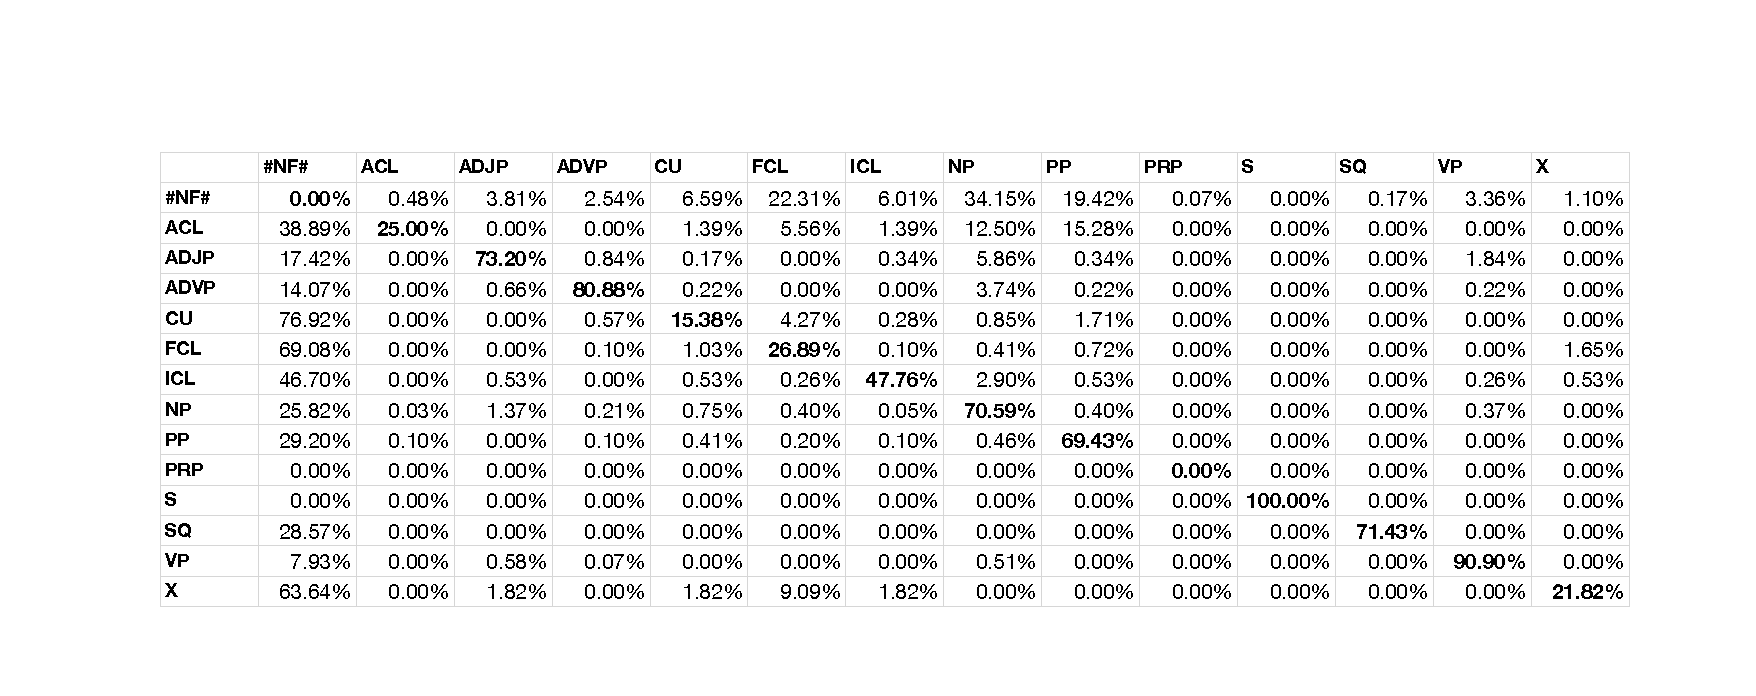
\includegraphics[scale=0.65]{score_confusion_cat.pdf}
	\caption{\label{confusion_matrix_cat} Matriz de Confusão: Categorias Sintáticas}		
  \end{center}
\end{figure}
